%% Please fill in your name and collaboration statement here.
\newcommand{\studentName}{Kevin Zhang}
\newcommand{\collaborationStatement}{I collaborated on this assignment with Tomoya Hasegawa, Jason Shen, and David DiCurcio, got help from no one else, and referred to http://madebyevan.com/fsm/ to draw automata.}


%%%%%%%%%%%%%%%%%%%%%%%%%%%%%%%%%%%%%%%%%%%%%%%
\documentclass[solution, letterpaper]{cs121}
\usepackage{tikz}
\usepackage{enumerate}
\begin{document}
\header{1}{Tuesday September 22, 2015 at 11:59pm}
\textit{Note: Finite automata (FA) drawings may be done by hand or using an online drawing tool.}
%%%%%%%%%%%%%%%%%%%%%%%%%%%%%%%%%%%%%%%%%%%%%%%
\PART{Sam and Serena}
%%%%%%%%%%%%%%%%%%%%%%%%%%%%%%%%%%%%%%%%%%%%%%%
\problem{2+2+1}{3 lines}

\includegraphics[width=7.0cm]{1-2a.png} \includegraphics[width=7.0cm]{1-2b.png}\\\\
\subproblem Describe informally $L_1$, the language accepted by the NFA on the left.\\
\subproblem Describe informally $L_2$, the language accepted by the NFA on the right.\\
\subproblem Write down $L_1 \cap L_2$.
\\\\
\noindent {\bf Solution.}
\\\\(A). $L_1$ is the language of all even-length strings of alternating $0$'s and $1$'s.
\\\\(B). $L_2$ is the language of all strings that consist of repeating $101$'s or $010$'s.  
\\\\(C). Since any string in $L_2$ longer than $3$ "letters" must be at least $6$ letters, and the first six letters of any string longer than $6$ letters in $L_2$ are either $010010$ or $101101$ (either repeating $101$'s or $010$'s), any string in $L_2$ six letters or longer cannot also be in $L_1$ (since there is either a repeating $0$ or a repeating $1$ in the string).  Therefore, the only strings that could potentially be in both $L_1$ and $L_2$ are those of length $3$ or $0$, or $\{010, 101, \vareps\}$.  However, since $L_1$ consists only of even-length strings, neither $101$ or $010$ can be in $L_1$.  Therefore, the only string in both $L_1$ and $L_2$ is $\vareps: L_1 \cap L_2 = \{\vareps\}$.

\problem{3+6+(2)}{1 page}
Let $S_n = \{1, 2, 3, ..., n\}$. We can represent subsets of $S_n$ using strings of length $n$ by setting the $i^{th}$ character to 1 if element $i$ is in the subset, and 0 if it is not. For example, for $n = 3$, the subset $\{3\}$ would be represented by the string $001$, and the subset $\{2, 3\}$ would be represented by the string $011$. Let $f_n : \{0, 1\}^n \to P(S_n) $ be a function that produces the subset represented by a string, e.g. $f_3(001) = \{3\}$ and $f_3(011) = \{2, 3\}$.

\subproblem Is $f_n$ injective for all $n$? Surjective? Bijective? Informally explain each of your answers.

\subproblem In this question, we will use the machinery of DFAs to ``compute'' a function. We will label accept states with values, and the state that the DFA halts at after processing an input string will correspond to the output of the function it computes. Your task is to draw a DFA that computes the function $f_3$. \textit{Notes: } 
\begin{itemize}
\item If the DFA is given a string of length greater than 3, it should enter a labeled ``error'' non-accept state. 
\item If the DFA is given a string of length 3, it should halt in an accept state that corresponds to the correct subset of $S_3$.  Thus you should have $2^3 = 8$ accept states. 
\item No additional explanation or description of the DFA is required beyond the drawing. 
\item Label the accept states in your drawing. An example of a labelled accept state that should appear in your drawing is below:\\
\includegraphics[width=3cm]{1-1ex.png}
\end{itemize}
\subproblem (Challenge!! Not required; worth up to 2 extra credit points.) How many states are required for a DFA that computes $f_n$? Prove that your answer is a lower bound.\\\\
\textit{Note: On every problem set we will provide a challenge problem, generally significantly more difficult than the other problems in the set, but worth only a few points. It is recommended that you attempt these problems, but only after completing the rest of the assignment.} 
\\\\
\noindent {\bf Solution.}
\\\\(A). $f_n$ is injective; if two length-$n$ strings result in the same sets, then they must have the exact same letters as well (if they differ at one place, the element which corresponds to that digit is in one set and not in the other).  $f_n$ is also surjective; it's easy to see that every subset of $S_n$ is representable by a string of $0$'s and $1$'s.  Thus, $f_n$ is bijective, since it is both injective and surjective.
\\\\(B).  Note: all transitions $0$'s and $1$'s leaving final states go to the error state (not drawn).
\\\begin{center}
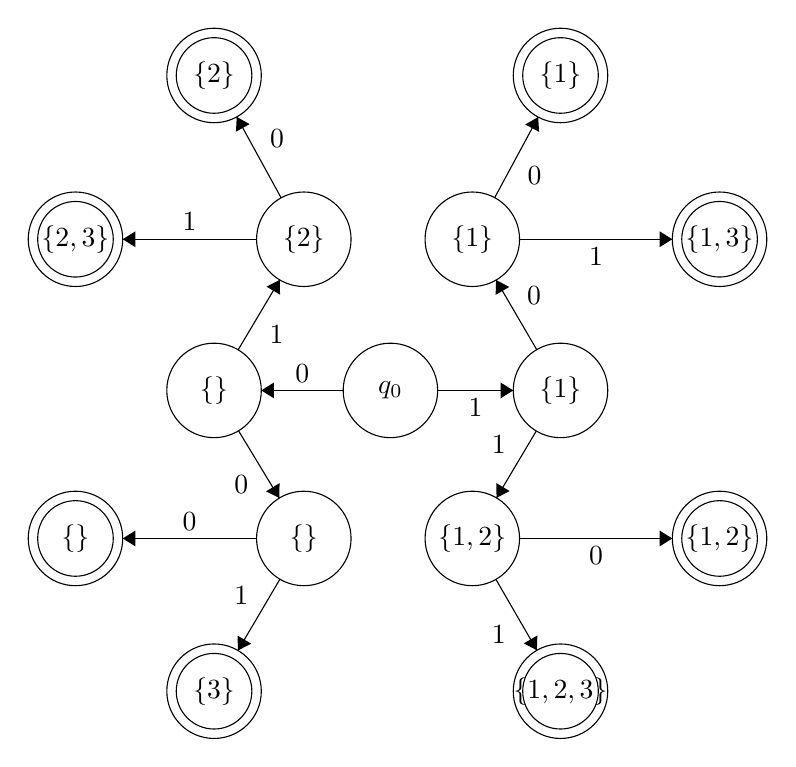
\begin{tikzpicture}[scale=0.2]
\tikzstyle{every node}+=[inner sep=0pt]
\draw [black] (39,-28.4) circle (3);
\draw (39,-28.4) node {$q_0$};
\draw [black] (49.8,-28.4) circle (3);
\draw (49.8,-28.4) node {$\{1\}$};
\draw [black] (27.8,-28.4) circle (3);
\draw (27.8,-28.4) node {$\{\}$};
\draw [black] (33.5,-18.8) circle (3);
\draw (33.5,-18.8) node {$\{2\}$};
\draw [black] (44.2,-37.8) circle (3);
\draw (44.2,-37.8) node {$\{1,2\}$};
\draw [black] (33.5,-37.8) circle (3);
\draw (33.5,-37.8) node {$\{\}$};
\draw [black] (44.2,-18.8) circle (3);
\draw (44.2,-18.8) node {$\{1\}$};
\draw [black] (27.8,-8.4) circle (3);
\draw (27.8,-8.4) node {$\{2\}$};
\draw [black] (27.8,-8.4) circle (2.4);
\draw [black] (59.9,-18.8) circle (3);
\draw (59.9,-18.8) node {$\{1,3\}$};
\draw [black] (59.9,-18.8) circle (2.4);
\draw [black] (19,-18.8) circle (3);
\draw (19,-18.8) node {$\{2,3\}$};
\draw [black] (19,-18.8) circle (2.4);
\draw [black] (27.8,-47.5) circle (3);
\draw (27.8,-47.5) node {$\{3\}$};
\draw [black] (27.8,-47.5) circle (2.4);
\draw [black] (19,-37.8) circle (3);
\draw (19,-37.8) node {$\{\}$};
\draw [black] (19,-37.8) circle (2.4);
\draw [black] (49.8,-47.5) circle (3);
\draw (49.8,-47.5) node {$\{1,2,3\}$};
\draw [black] (49.8,-47.5) circle (2.4);
\draw [black] (59.9,-37.8) circle (3);
\draw (59.9,-37.8) node {$\{1,2\}$};
\draw [black] (59.9,-37.8) circle (2.4);
\draw [black] (49.8,-8.4) circle (3);
\draw (49.8,-8.4) node {$\{1\}$};
\draw [black] (49.8,-8.4) circle (2.4);
\draw [black] (36,-28.4) -- (30.8,-28.4);
\fill [black] (30.8,-28.4) -- (31.6,-28.9) -- (31.6,-27.9);
\draw (33.4,-27.9) node [above] {$0$};
\draw [black] (42,-28.4) -- (46.8,-28.4);
\fill [black] (46.8,-28.4) -- (46,-27.9) -- (46,-28.9);
\draw (44.4,-28.9) node [below] {$1$};
\draw [black] (29.36,-30.97) -- (31.94,-35.23);
\fill [black] (31.94,-35.23) -- (31.96,-34.29) -- (31.1,-34.81);
\draw (30.01,-34.37) node [left] {$0$};
\draw [black] (29.33,-25.82) -- (31.97,-21.38);
\fill [black] (31.97,-21.38) -- (31.13,-21.81) -- (31.99,-22.32);
\draw (31.3,-24.85) node [right] {$1$};
\draw [black] (48.26,-30.98) -- (45.74,-35.22);
\fill [black] (45.74,-35.22) -- (46.57,-34.79) -- (45.72,-34.28);
\draw (46.36,-31.84) node [left] {$1$};
\draw [black] (48.29,-25.81) -- (45.71,-21.39);
\fill [black] (45.71,-21.39) -- (45.68,-22.33) -- (46.55,-21.83);
\draw (47.65,-22.36) node [right] {$0$};
\draw [black] (32.06,-16.17) -- (29.24,-11.03);
\fill [black] (29.24,-11.03) -- (29.19,-11.97) -- (30.06,-11.49);
\draw (31.32,-12.41) node [right] {$0$};
\draw [black] (47.2,-18.8) -- (56.9,-18.8);
\fill [black] (56.9,-18.8) -- (56.1,-18.3) -- (56.1,-19.3);
\draw (52.05,-19.3) node [below] {$1$};
\draw [black] (30.5,-18.8) -- (22,-18.8);
\fill [black] (22,-18.8) -- (22.8,-19.3) -- (22.8,-18.3);
\draw (26.25,-18.3) node [above] {$1$};
\draw [black] (31.98,-40.39) -- (29.32,-44.91);
\fill [black] (29.32,-44.91) -- (30.16,-44.48) -- (29.29,-43.97);
\draw (30,-41.4) node [left] {$1$};
\draw [black] (30.5,-37.8) -- (22,-37.8);
\fill [black] (22,-37.8) -- (22.8,-38.3) -- (22.8,-37.3);
\draw (26.25,-37.3) node [above] {$0$};
\draw [black] (45.7,-40.4) -- (48.3,-44.9);
\fill [black] (48.3,-44.9) -- (48.33,-43.96) -- (47.47,-44.46);
\draw (46.35,-43.88) node [left] {$1$};
\draw [black] (47.2,-37.8) -- (56.9,-37.8);
\fill [black] (56.9,-37.8) -- (56.1,-37.3) -- (56.1,-38.3);
\draw (52.05,-38.3) node [below] {$0$};
\draw [black] (45.62,-16.16) -- (48.38,-11.04);
\fill [black] (48.38,-11.04) -- (47.56,-11.51) -- (48.44,-11.98);
\draw (47.68,-14.77) node [right] {$0$};
\end{tikzpicture}
\end{center}
(C).  The initial state counts for 1 state; after reading each input, twice as many states are possible (i.e. 2 states are possible after the first input, 4 after the second, and so on).  No set can count for more than one state (i.e. the empty set $\{\}$ cannot count for both intermediate states while reading 001 or 010), because we need to keep track of the inputs leading up to that point to make sure we read no more than $n$ letters.  In addition, there is at least one error state.  Therefore, we have the sum $\underset{i=0}{\overset{n}{\Sigma}}2^i + 1 = 2^{n+1}$ minimum states.
%%%%%%%%%%%%%%%%%%%%%%%%%%%%%%%%%%%%%%%%%%%%%%%
\PART{Juan and Varun}
%%%%%%%%%%%%%%%%%%%%%%%%%%%%%%%%%%%%%%%%%%%%%%%
\problem{5+5}{1/2 page}

Two FAs are ``equivalent'' if the languages that they accept are the same. If two FAs are not equivalent, they are ``distinct''. For this question, you may assume that the alphabet is $\{0, 1\}$.

\subproblem How many distinct DFAs are there with 1 state? Draw it/them. Describe informally the languages recognized by each.

\subproblem How many distinct NFAs are there with 1 state? Draw it/them. Describe informally the languages recognized by each.
\\\\
\noindent {\bf Solution.}
\\\\(A). There are two DFAs with only one state; one that accepts all strings (including the empty string), and one that rejects all strings (including the empty string).

\begin{center}
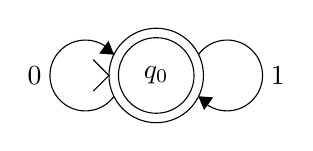
\begin{tikzpicture}[scale=0.2]
\tikzstyle{every node}+=[inner sep=0pt]
\draw [black] (0,0) circle (3);
\draw (0,0) node {$q_0$};
\draw [black] (0,0) circle (2.4);
\draw (-4,1) -- (-3,0) -- (-4,-1);
\draw [black] (-2.68,-1.323) arc (-36:-324:2.25);
\draw (-7.25,0) node [left] {$0$};
\fill [black] (-2.68,1.32) -- (-3.03,2.2) -- (-3.62,1.39);
\draw [black] (2.68,1.323) arc (144:-144:2.25);
\draw (7.25,0) node [right] {$1$};
\fill [black] (2.68,-1.32) -- (3.03,-2.2) -- (3.62,-1.39);
\end{tikzpicture}
\hspace{0.4cm}
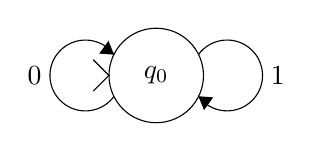
\begin{tikzpicture}[scale=0.2]
\tikzstyle{every node}+=[inner sep=0pt]
\draw [black] (0,0) circle (3);
\draw (0,0) node {$q_0$};
\draw (-4,1) -- (-3,0) -- (-4,-1);
\draw [black] (-2.68,-1.323) arc (-36:-324:2.25);
\draw (-7.25,0) node [left] {$0$};
\fill [black] (-2.68,1.32) -- (-3.03,2.2) -- (-3.62,1.39);
\draw [black] (2.68,1.323) arc (144:-144:2.25);
\draw (7.25,0) node [right] {$1$};
\fill [black] (2.68,-1.32) -- (3.03,-2.2) -- (3.62,-1.39);
\end{tikzpicture}
\end{center}

\noindent(B). There are five NFAs with exactly 1 state; they are diagrammed below. 
\begin{itemize}
	\setlength\itemsep{0cm}
	\item The first accepts any string of $0$'s and $1$'s, including the empty string,
	\item the second accepts only the empty string and strings of $1$'s,
	\item the third accepts only the empty string and strings of $0$'s,
	\item the fourth accepts only the empty string, and 
	\item the fifth accepts no strings at all.
\end{itemize}

\begin{center}
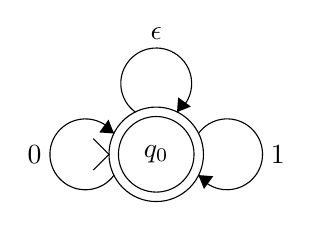
\begin{tikzpicture}[scale=0.2]
\tikzstyle{every node}+=[inner sep=0pt]
\draw [black] (0,0) circle (3);
\draw (0,0) node {$q_0$};
\draw [black] (0,0) circle (2.4);
\draw (-4,1) -- (-3,0) -- (-4,-1);
\draw [black] (-2.68,-1.323) arc (-36:-324:2.25);
\draw (-7.25,0) node [left] {$0$};
\fill [black] (-2.68,1.32) -- (-3.03,2.2) -- (-3.62,1.39);
\draw [black] (2.68,1.323) arc (144:-144:2.25);
\draw (7.25,0) node [right] {$1$};
\fill [black] (2.68,-1.32) -- (3.03,-2.2) -- (3.62,-1.39);
\draw [black] (-1.323,2.68) arc (234:-54:2.25);
\draw (0.0,7.25) node [above] {$\epsilon$};
\fill [black] (1.32,2.68) -- (2.2,3.03) -- (1.39,3.62);
\end{tikzpicture}
\hspace{0.4cm}
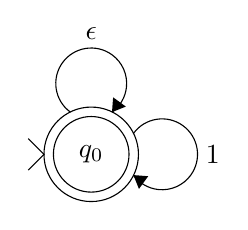
\begin{tikzpicture}[scale=0.2]
\tikzstyle{every node}+=[inner sep=0pt]
\draw [black] (0,0) circle (3);
\draw (0,0) node {$q_0$};
\draw [black] (0,0) circle (2.4);
\draw (-4,1) -- (-3,0) -- (-4,-1);
\draw [black] (2.68,1.323) arc (144:-144:2.25);
\draw (7.25,0) node [right] {$1$};
\fill [black] (2.68,-1.32) -- (3.03,-2.2) -- (3.62,-1.39);
\draw [black] (-1.323,2.68) arc (234:-54:2.25);
\draw (0.0,7.25) node [above] {$\epsilon$};
\fill [black] (1.32,2.68) -- (2.2,3.03) -- (1.39,3.62);
\end{tikzpicture}
\hspace{0.4cm}
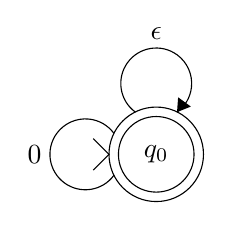
\begin{tikzpicture}[scale=0.2]
\tikzstyle{every node}+=[inner sep=0pt]
\draw [black] (0,0) circle (3);
\draw (0,0) node {$q_0$};
\draw [black] (0,0) circle (2.4);
\draw (-4,1) -- (-3,0) -- (-4,-1);
\draw [black] (-2.68,-1.323) arc (-36:-324:2.25);
\draw (-7.25,0) node [left] {$0$};
\draw [black] (-1.323,2.68) arc (234:-54:2.25);
\draw (0.0,7.25) node [above] {$\epsilon$};
\fill [black] (1.32,2.68) -- (2.2,3.03) -- (1.39,3.62);
\end{tikzpicture}
\hspace{0.4cm}
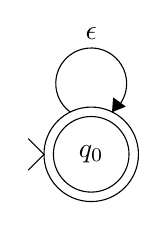
\begin{tikzpicture}[scale=0.2]
\tikzstyle{every node}+=[inner sep=0pt]
\draw [black] (0,0) circle (3);
\draw (0,0) node {$q_0$};
\draw [black] (0,0) circle (2.4);
\draw (-4, 1) -- (-3, 0) -- (-4, -1);
\draw [black] (-1.323,2.68) arc (234:-54:2.25);
\draw (0.0,7.25) node [above] {$\epsilon$};
\fill [black] (1.32,2.68) -- (2.2,3.03) -- (1.39,3.62);
\end{tikzpicture}
\hspace{0.4cm}
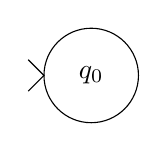
\begin{tikzpicture}[scale=0.2]
\tikzstyle{every node}+=[inner sep=0pt]
\draw [black] (0,0) circle (3);
\draw (0,0) node {$q_0$};
\draw (-4, 1) -- (-3, 0) -- (-4, -1);
\end{tikzpicture}
\end{center}

\problem{3+3+3}{1/3 page}
Are the following statements true or false? Justify your answers with a proof or counterexample.\\
\subproblem $(L_1 \cap L_2)^* = L_1^* \cap L_2^*$

\subproblem $(L_1 \cup L_2) \cdot L_3 = (L_1 \cdot L_3) \cup (L_2 \cdot L_3)$, where $\cdot$ is concatenation.

\subproblem $\{ \vareps\} \cdot L_1 = \emptyset \cdot L_1$
\\\\
\noindent {\bf Solution.}
\\\\(A). $\textbf{False}$.  Let $L_1$ be $\{1,0\}$ and $L_2$ be $\{10\}$.  The left side is just $\emptyset^*$, while the right side at least contains 10.
\\\\(B). $\textbf{True}$.  Let $s \in (L_1 \cup L_2) \cdot L_3$.  Let elements of $L_1$ be denoted as $a_i$ for some $i$, elements of $L_2$ be denoted as $b_k$ for some $k$, and elements of $L_3$ be denoted as $c_j$ for some $j$.  Then $s$ is either of the format $(a_i)^* \cdot (c_j)^*$ or $(b_i)^* \cdot (c_j)^*$.  The former case is an element of $(L_1 \cdot L_3)$, while the latter is an element of $(L_2 \cdot L_3)$.  Thus, every element in $(L_1 \cup L_2) \cdot L_3$ is also in $(L_1 \cdot L_3) \cup (L_2 \cdot L_3)$.
\\\indent We also need to prove that if $s \in (L_1 \cdot L_3) \cup (L_2 \cdot L_3)$, then $s \in (L_1 \cup L_2) \cdot L_3$.  This is straightforward to see; in either case (whether $s \in (L_1 \cdot L_3)$ or $s \in (L_2 \cdot L_3)$), $s$ is composed of either a string of $a_i$ or $b_j$ and a string of $c_j$.  This means that $s$ can be divided into a substring that is either in $L_1$ or $L_2$, and a substring that is in $L_3$.  This is exactly $(L_1 \cup L_2) \cdot L_3$.
\\\\(C). $\textbf{False}$.  The left side consists of $L_1$ itself; prepending any element of $L_1$ by the only element in $\{\vareps\}$, $\vareps$ does nothing.  However, the right side consists of no elements at all, since the empty set contains nothing and therefore there is nothing to concatenate.  These two sets are obviously not equal.
\end{document}